\section{Monopole Antenna -- Prototype}
The first monopole prototype can be seen in Figure \ref{fig:ant1_proto1_3d}. As seen on the figure both monopole antennas were very fragile. The feed pads were too small and fragile, which caused them to brake off, also as seen on the figure.

To solve the feed pad problem, a new prototype was made with $\SI{10}{mm}\times \SI{2.5}{mm}$ feed pads. The pad size was chosen to match the final tuning PCB for the project. Furthermore a FR4 support was added under the antenna feeds to make it more robust. The new prototype can be seen in Figure \ref{fig:ant1_proto2_3d}.

\begin{figure}[htbp]
   \begin{subfigure}[b]{0.49\linewidth}
        \centering
        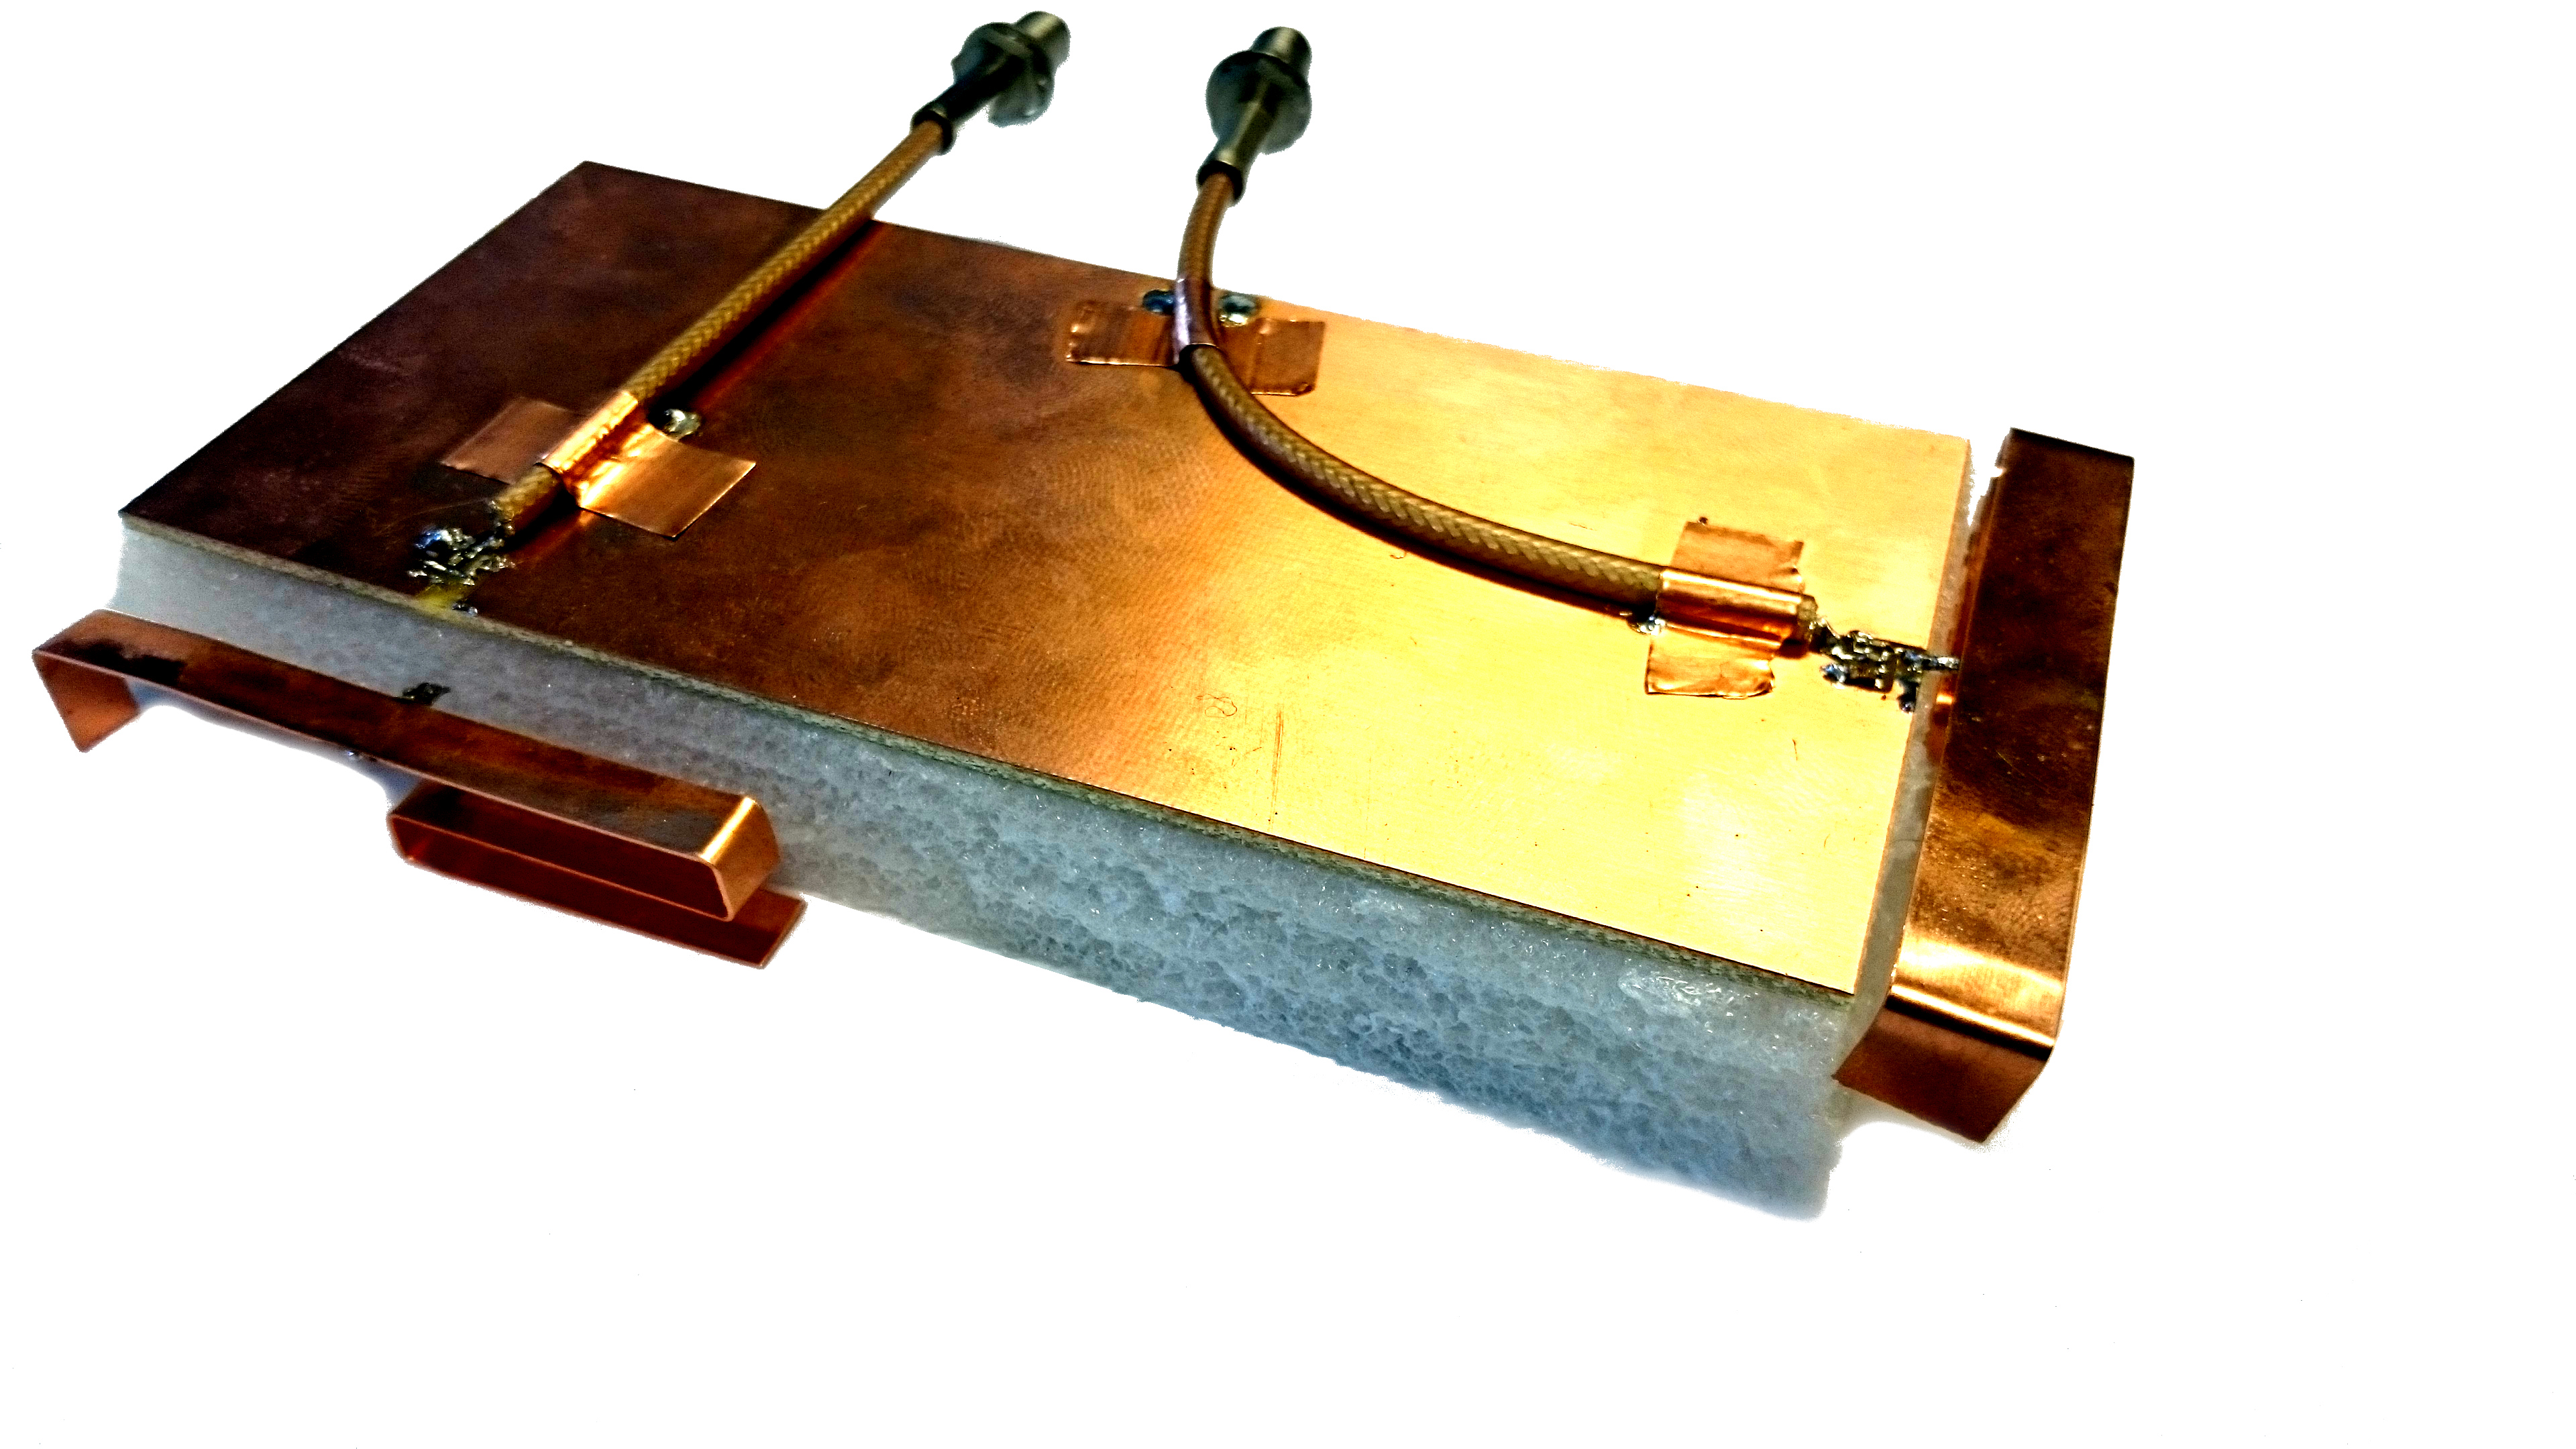
\includegraphics[scale=0.2]{img/tech_sol/monopole/prototype_v1/monopole_v1}
        \caption{Monopole prototype version 1}
        \label{fig:ant1_proto1_3d}
    \end{subfigure}
    \hfill
    \begin{subfigure}[b]{0.49\linewidth}
        \centering
        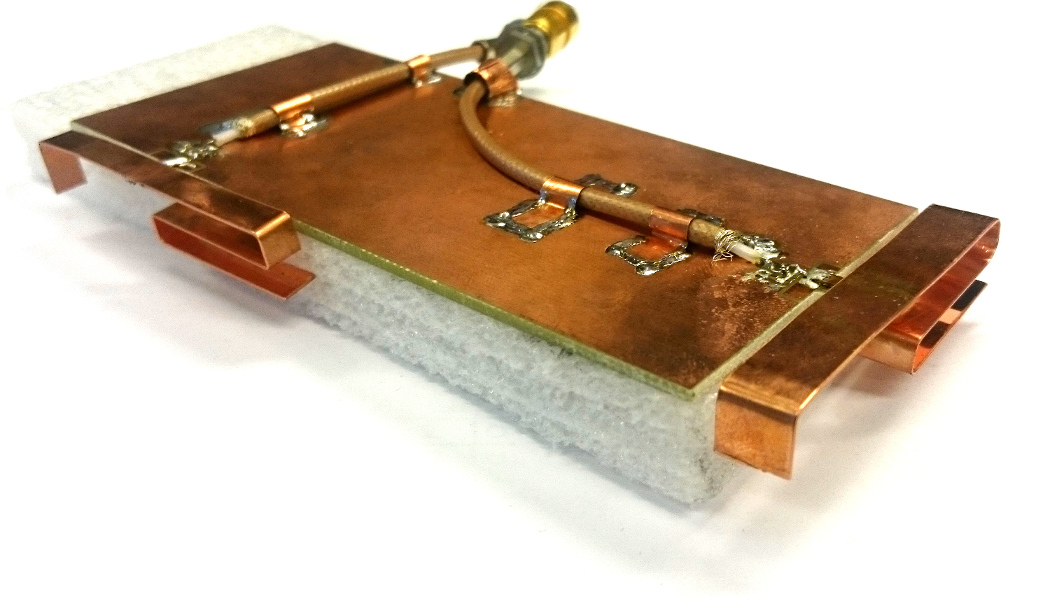
\includegraphics[scale=0.27]{img/tech_sol/monopole/prototype_v2/monopole_v2}
        \caption{Monopole prototype version 2}
        \label{fig:ant1_proto2_3d}
    \end{subfigure}
    \caption{Monopole prototype comparison of version 1 and 2}
    \label{fig:ant_1_proto_3d}
\end{figure}

\FloatBarrier
\subsection{Simulation}
The second prototype had some small changes of the feed pad and fr4 support, as described above. As a result the matching deviated some in comparison with version 1 matching simulations, which can be seen in Figure \ref{fig:sparam_mono_free_space}. To compensate for the design changes, the component values was changes accordingly. The new component values can be seen in Table \ref{fig:mono_proto_sim_matching}.

\begin{figure}[htbp]
        \centering
        \begin{tabular}{m{3in}m{3in}}
            \centering
            \includegraphics{img/tech_sol/schematic_tuning_1}&
            \centering
            \footnotesize
            \begin{tabular}{|l|l|l|l|}
                \hline
                & $C_1$ & $L_1$ & $C_2$ \\
                \hline
                Top antenna & \SI{6.5}{pF} & \SI{7}{nH} & \SI{0.3}{pF} \\
                Side antenna & \SI{2.7}{pF} & \SI{4.9}{nH} & \SI{0.3}{pF} \\
                \hline
            \end{tabular}
        \end{tabular}
    \caption{Matching circuit for the simulation prototype monopole antenna. These are the component values where the bandwidth is found to be the largest.}
    \label{fig:mono_proto_sim_matching}
\end{figure}

The S-parameters of the prototype can be seen on Figure \ref{fig:sparam_mono_proto_sim}. In comparison with version 1 S-parameter S11 and S22, the spectrum coverage for the top antenna has been slightly improved. The improvement is significant in the high band, where the top antenna now covers from \SI{1500}{MHz} to \SI{3000}{MHz}, only with a small decrease of \SI{-1}{dB} around \SI{2500}{MHz.}. The side antenna also shows spectrum improvement in the high band, but lacks some coverage of approx \SI{-3}{dB} from \SI{1710}{MHz} to \SI{1800}{MHz}. Generally the low band coverage for both antennas compared with version 1, have decreased but still covers the band.

\fixme{efficiency ddocumentation}
\begin{figure}[htbp]
   \begin{subfigure}[b]{0.49\linewidth}
        \centering
        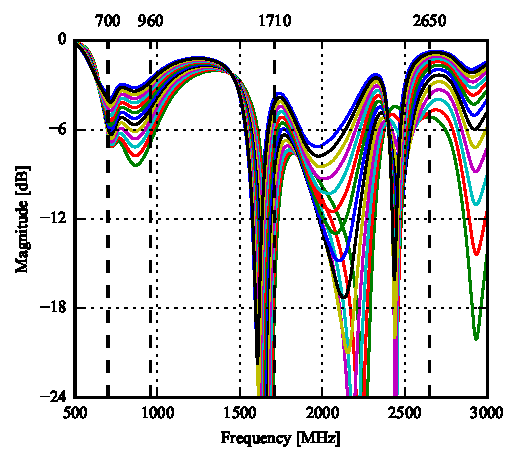
\includegraphics{img/tech_sol/monopole/prototype_v2/sim_s11}
        \caption{$S_{11}$, sweeping $C_1$ and fixing $C_2$.}
        \label{fig:ant1_proto_sim_s11}
    \end{subfigure}
    \hfill
    \begin{subfigure}[b]{0.49\linewidth}
        \centering
        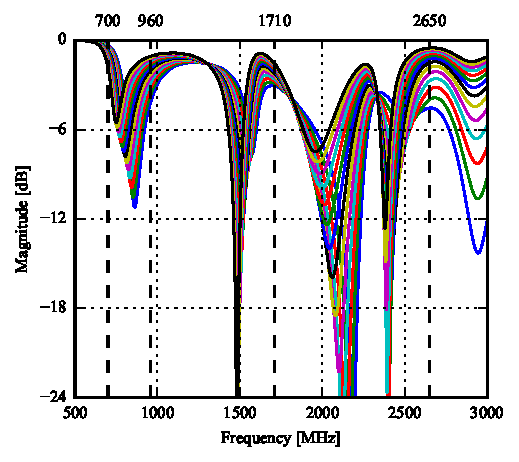
\includegraphics{img/tech_sol/monopole/prototype_v2/sim_s22}
        \caption{$S_{22}$, sweeping $C_2$ and fixing $C_1$.}
        \label{fig:ant1_proto_sim_s22}
    \end{subfigure}
~
    \begin{subfigure}[b]{0.49\linewidth}
        \centering
        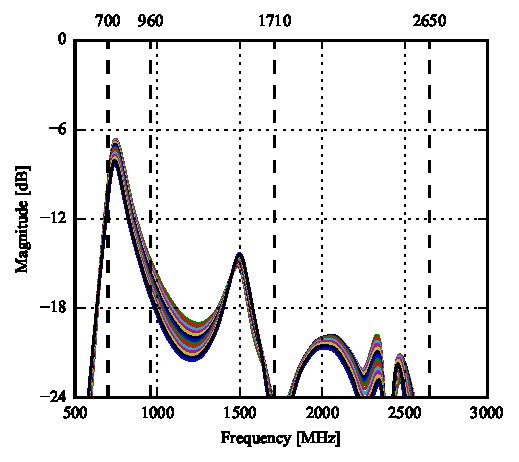
\includegraphics{img/tech_sol/monopole/prototype_v2/sim_s12_s11}
        \caption{$S_{21}$, sweeping $C_1$ and fixing $C_2$.}
        \label{fig:ant1_proto_sim_s11_s12}
    \end{subfigure}
    \hfill
    \begin{subfigure}[b]{0.49\linewidth}
        \centering
        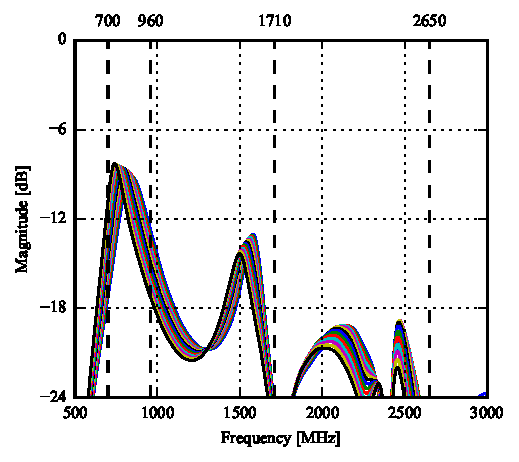
\includegraphics{img/tech_sol/monopole/prototype_v2/sim_s12_s22}
        \caption{$S_{21}$, sweeping $C_2$ and fixing $C_1$.}
        \label{fig:ant1_proto_sim_s22_s12}
    \end{subfigure}
    \caption{S-parameter sweep in free space for tuning the shunt capacitor of each antenna, $C_1$ and $C_2$ for port 1 and 2, respectively. Port 1 is the top antenna and port 2 is the side antenna.}
    \label{fig:sparam_mono_proto_sim}
\end{figure}

\FloatBarrier
\subsection{Measurements}
A comparison between the simulated and measured s-parameters and efficiencies can be seen on Figure \ref{fig:mono_proto_sparam_eff}. The simulated and measured results are done with the tunable capacitor at \SI{0.3}{pF}. Furthermore some component changes were made going from simulation to the prototype, these can be seen in Table \ref{fig:mono_proto_meas_matching}

\begin{figure}[htbp]
        \centering
        \begin{tabular}{m{3in}m{3in}}
            \centering
            \includegraphics{img/tech_sol/schematic_tuning_1}&
            \centering
            \footnotesize
            \begin{tabular}{|l|l|l|l|}
                \hline
                & $C_1$ & $L_1$ & $C_2$ \\
                \hline
                Top antenna & \SI{2.2}{pF} & \SI{3.3}{nH} & \SI{0.3}{pF} \\
                Side antenna & \SI{3.3}{pF} & \SI{1.2}{nH} & \SI{0.3}{pF} \\
                \hline
            \end{tabular}
        \end{tabular}
    \caption{Matching circuit for the measured prototype monopole antenna. These are the component values where the bandwidth is found to be the largest.}
    \label{fig:mono_proto_meas_matching}
\end{figure}

\begin{figure}[htbp]
    \centering
    \begin{subfigure}{0.49\linewidth}
        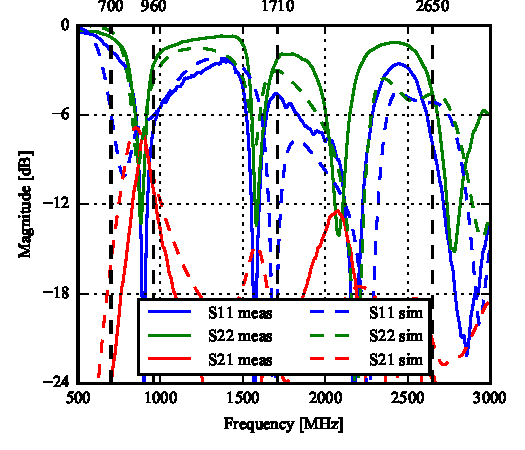
\includegraphics{img/tech_sol/monopole/prototype_v2/sparams.pdf}
        \caption{S-parameters.}
    \end{subfigure}
    \hfill
    \begin{subfigure}{0.49\linewidth}
        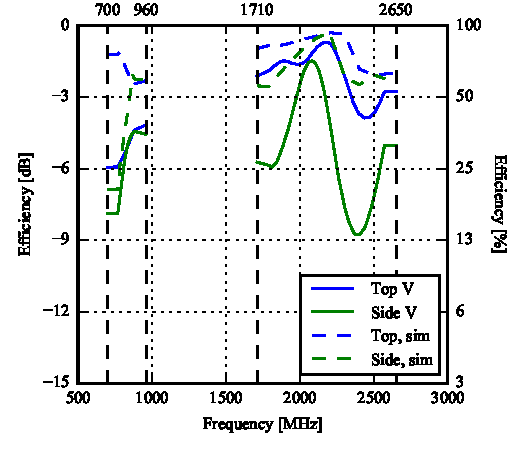
\includegraphics{img/tech_sol/monopole/prototype_v2/efficiency.pdf}
        \caption{Total efficiency.}
    \end{subfigure}
    \caption{S-parameters and total efficiency of the monopole antenna prototype with the component values from Figure~\ref{fig:mono_proto_sim_matching}.}
    \label{fig:mono_proto_sparam_eff}
\end{figure}

\begin{figure}[htbp]
   \begin{subfigure}[b]{0.49\linewidth}
        \centering
        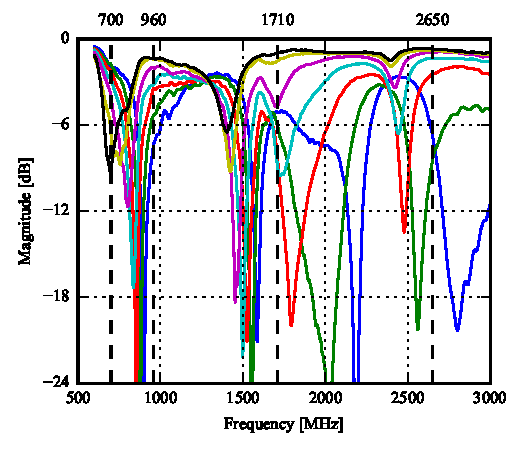
\includegraphics{img/tech_sol/monopole/prototype_v2/meas_s11_csh1}
        \caption{$S_{11}$, sweeping $C_1$ and fixing $C_2$.}
        \label{fig:ant1_proto_sim_s11}
    \end{subfigure}
    \hfill
    \begin{subfigure}[b]{0.49\linewidth}
        \centering
        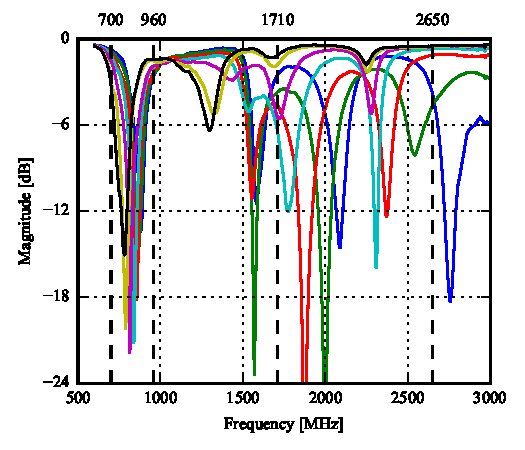
\includegraphics{img/tech_sol/monopole/prototype_v2/meas_s22_csh2}
        \caption{$S_{22}$, sweeping $C_2$ and fixing $C_1$.}
        \label{fig:ant1_proto_sim_s22}
    \end{subfigure}
~
    \begin{subfigure}[b]{0.49\linewidth}
        \centering
        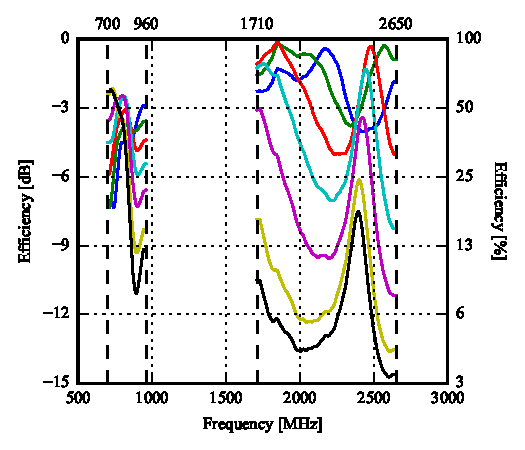
\includegraphics{img/tech_sol/monopole/prototype_v2/meas_efficiency_top}
        \caption{$S_{21}$, sweeping $C_1$ and fixing $C_2$.}
        \label{fig:ant1_proto_sim_s11}
    \end{subfigure}
    \hfill
    \begin{subfigure}[b]{0.49\linewidth}
        \centering
        \includegraphics{img/tech_sol/monopole/prototype_v2/meas_efficiency}
        \caption{$S_{21}$, sweeping $C_2$ and fixing $C_1$.}
        \label{fig:ant1_proto_sim_s22}
    \end{subfigure}
    \caption{S-parameter sweep in free space for tuning the shunt capacitor of each antenna, $C_1$ and $C_2$ for port 1 and 2, respectively. Port 1 is the top antenna and port 2 is the side antenna.}
    \label{fig:sparam_mono_proto_sim}
\end{figure}